%% Label-Free Score Calibration for Cross-Domain Animal Re-ID
%% Target: IJCB / WACV. Compiles with IEEEtran (ships with all TeX distros; Overleaf-ready).
%% Contribution is empirical/analytical (a conditional characterization), not a new method.
\documentclass[conference]{IEEEtran}
\IEEEoverridecommandlockouts
\usepackage{cite}
\usepackage{amsmath,amssymb,amsfonts}
\usepackage{graphicx}
\usepackage{booktabs}
\usepackage{array}
\usepackage{xcolor}
\usepackage[hidelinks]{hyperref}
\usepackage{url}

\begin{document}

\title{When Does Label-Free Score Calibration Recover\\ Cross-Domain Animal Re-Identification?}

\author{\IEEEauthorblockN{Anonymous Submission}
\IEEEauthorblockA{Paper ID: XXXX}}

\maketitle

\begin{abstract}
Foundation models for animal re-identification (re-ID), such as MegaDescriptor, achieve
near-perfect verification on species and datasets seen during training, yet degrade sharply under
domain shift---new farms, sessions, cameras, or unseen distributions. We ask a narrow but practical
question: \emph{when} is this degradation recoverable without labels, retraining, or access to
source data, simply by recalibrating similarity scores at test time? Across three backbones
(a task-specific muzzle CNN, the re-ID foundation model MegaDescriptor-L, and the general-purpose
self-supervised model DINOv2), four biometric modalities (cattle muzzle, primate face, cattle coat,
panda coat pattern), and three families of domain shift (cross-dataset transfer, controlled image
corruption, and natural cross-session splits), we show that cross-domain verification loss is
primarily a problem of \emph{score mis-calibration} rather than feature quality, and that adaptive
symmetric score normalization (S-norm) recovers a statistically significant fraction of it at zero
training cost. Crucially, we characterize \emph{when} it helps: the recovery scales with a
measurable mis-calibration signal (the baseline equal-error rate, EER). In a controlled comparison on
identical data and shift, a backbone well-calibrated for the target species shows no gap and no
benefit, whereas a general backbone mis-calibrated for re-ID degrades by over twelve EER points and
is significantly recovered by the same calibration step. Feature-level test-time adaptation (AdaBN)
is, by contrast, unreliable. Score-level calibration is thus a dependable, deployable baseline for
cross-domain animal re-ID, and its applicability is predictable in advance.
\end{abstract}

\begin{IEEEkeywords}
animal re-identification, test-time adaptation, score normalization, cross-domain generalization,
biometrics, calibration.
\end{IEEEkeywords}

\section{Introduction}
Individual animal re-identification (re-ID) underpins ecological monitoring, precision livestock
farming, and anti-poaching. The field has converged on large pretrained embedding models:
MegaDescriptor~\cite{cermak2024}, trained on 2.8M images spanning 30k identities and 33 species, is
the de-facto state of the art and outperforms general vision backbones such as CLIP and
DINOv2~\cite{oquab2024} on in-domain benchmarks. The community's most-cited open problem, however,
is generalization: on cross-domain or time/similarity-aware splits, even MegaDescriptor drops by
tens of points, because ecological data is collected under conditions that differ from training.

Test-time adaptation (TTA) is the natural remedy, but most methods operate on \emph{features}
(e.g., batch-norm statistics~\cite{li2017}, entropy minimization~\cite{wang2021}) and require
gradient steps or careful tuning; in re-ID they can be unstable when the target set is
small~\cite{dart2025}. We take a deliberately minimal view. Under domain shift the \emph{ranking} of
a re-ID model often survives---the correct identity is still near the top---while the \emph{operating
threshold} that separates genuine from impostor pairs does not transfer. This is a calibration
failure of the score distribution, not a collapse of the features.

This paper is an empirical and analytical study of one consequence: adaptive symmetric score
normalization (S-norm)~\cite{auckenthaler2000}, a technique from speaker verification, can be applied
verbatim at test time---no labels, no retraining, no source data---to realign the score distribution
to the target domain. Our contributions are:
\begin{enumerate}
\item A broad, honest empirical demonstration that S-norm recovers cross-domain re-ID verification
across three backbones, four biometric modalities, and three shift families.
\item A conditional characterization with significance testing. Using probe-level bootstrap
confidence intervals, we show the recovery is significant precisely when the score distribution is
mis-calibrated (large baseline EER) and negligible otherwise, and we give a controlled two-backbone
comparison on identical data that isolates calibration as the cause.
\item Evidence that the fix is score-level, not feature-level: feature-level AdaBN is unreliable
(helping on some sets, destabilizing others), whereas score-level S-norm is monotone-safe.
\end{enumerate}
We are explicit that this is \emph{not} a new method: we tested adaptive top-$k$ (AS-norm), quantile
normalization, and a quality-conditioned variant, and none robustly beats plain S-norm. The value of
the paper is the characterization---telling practitioners when a zero-cost baseline will and will not
help.

\section{Related Work}
\textbf{Foundation models for animal re-ID.} MegaDescriptor and the WildlifeDatasets
toolkit~\cite{cermak2024} standardized large-scale animal re-ID; WildlifeReID-10k~\cite{adam2024}
(10k identities, 33 species) established leakage-aware, time/similarity-aware evaluation. These works
document, but do not resolve, the cross-domain gap.

\textbf{Test-time adaptation.} TENT~\cite{wang2021}, AdaBN~\cite{li2017}, and vision-language TTA
adapt features or predictions at test time; DART$^3$~\cite{dart2025} studies TTA for person re-ID.
Most require adaptation steps and can be brittle with few target samples; our approach needs neither
gradients nor labels.

\textbf{Score normalization.} Z-norm, T-norm, and (adaptive) S-norm~\cite{auckenthaler2000} originate
in speaker verification as cohort-based recalibration of verification scores. Quality-based score
fusion~\cite{nandakumar2006} weights modalities by input quality. We repurpose S-norm as a
domain-adaptation tool for visual re-ID and, unlike prior fusion work, characterize \emph{when} it is
statistically effective.

\section{Method}
\textbf{Setup.} Given a gallery of enrolled templates and a set of probes, a backbone produces
$\ell_2$-normalized embeddings; the score matrix $S$ holds cosine similarities between probes (rows)
and gallery templates (columns). Verification thresholds $S$; identification ranks each row.

\textbf{Adaptive symmetric S-norm.} For probe $i$ and template $j$,
\begin{equation}
S'_{ij} = \tfrac{1}{2}\!\left[\frac{S_{ij}-\mu_i}{\sigma_i} + \frac{S_{ij}-\mu_j}{\sigma_j}\right],
\end{equation}
where $(\mu_i,\sigma_i)$ are the mean and standard deviation of probe $i$'s scores against the
gallery cohort, and $(\mu_j,\sigma_j)$ those of template $j$ against the probe cohort. The cohort is
the target set itself; no labels or source data are used. Intuitively, S-norm removes per-probe and
per-template offsets/scales that domain shift introduces, restoring a common operating point.

\textbf{Mis-calibration predictor.} We use the baseline EER (equivalently, the overlap of the genuine
and impostor score distributions) as an a-priori indicator of whether S-norm will help: a large
baseline EER signals a mis-calibrated distribution with headroom for recalibration.

\textbf{Baselines.} (i) Raw cosine; (ii) AdaBN~\cite{li2017} (feature-level BN-statistic adaptation);
(iii) alternative score-norms---AS-norm (top-$k$ cohort), quantile/rank normalization, and a
quality-conditioned S-norm that scales calibration strength per probe by a confidence signal.

\section{Experimental Setup}
\textbf{Backbones.} (a) a task-specific EfficientNet-B4 + ArcFace~\cite{deng2019} muzzle CNN trained
on a single cattle dataset; (b) MegaDescriptor-L-384; (c) DINOv2 ViT-B/14, used as a frozen embedding
extractor.

\textbf{Datasets / modalities.} Cattle muzzle (two external cross-datasets), MacaqueFaces (primate
face), CZoo (chimpanzee face), FriesianCattle2017 (cattle coat), IPanda50 (panda pattern).

\textbf{Domain-shift protocols.} (i) \emph{Cross-dataset}: train on one cattle dataset, enroll and
probe a different one. (ii) \emph{Corruption}: clean gallery, probes corrupted with blur/brightness/
spatter at graded severities. (iii) \emph{Natural}: split gallery/probe by metadata---MacaqueFaces by
capture date (temporal), IPanda50 by video (recording session)---an ecologically valid shift with no
synthetic manipulation.

\textbf{Metrics and significance.} Verification EER and ROC-AUC. For each condition we report the EER
recovery (baseline minus S-norm) with a 95\% bootstrap confidence interval over resampled probes;
``significant'' means the interval excludes zero.

\begin{table*}[t]
\centering
\caption{S-norm recovery across backbones, modalities, and shift families. Recovery is the EER
reduction (baseline $-$ S-norm), with 95\% probe-level bootstrap CI where computed. The benefit is
significant precisely in the mis-calibrated (large baseline EER) regime.}
\label{tab:main}
\begin{tabular}{@{}lllccrl@{}}
\toprule
Backbone & Modality & Shift & Baseline EER & +S-norm & Recovery & 95\% CI / note \\
\midrule
Muzzle CNN (ours) & cattle muzzle & cross-dataset (308 IDs) & 12.2\% & 7.9\% & $+4.0$ pt & $[+3.2,+4.7]$ \textbf{sig} \\
Muzzle CNN (ours) & cattle muzzle & cross-dataset (24 IDs) & 14.8\% & 11.4\% & $+3.4$ pt & large-EER regime \\
MegaDescriptor-L & macaque face & corruption (spatter) & 6.24\% & 5.34\% & $+0.9$ pt & large-EER regime \\
MegaDescriptor-L & Friesian coat & corruption (spatter) & 2.77\% & 1.15\% & $+1.6$ pt & large-EER regime \\
MegaDescriptor-L & panda pattern & natural (cross-video) & 2.63\% & 2.29\% & $-0.04$ pt & $[-0.33,+0.14]$ \textbf{n.s.} \\
MegaDescriptor-L & macaque face & natural (date) & 0.08\% & 0.08\% & $0$ & no gap \\
DINOv2 (general) & panda pattern & natural (cross-video) & 40.8\% & 35.3\% & $+5.5$ pt & $[+4.0,+7.2]$ \textbf{sig} \\
DINOv2 (general) & macaque face & natural (date) & 29.2\% & 20.7\% & $+8.4$ pt & $[+7.2,+9.8]$ \textbf{sig} \\
\bottomrule
\end{tabular}
\end{table*}

\begin{figure}[t]
\centering
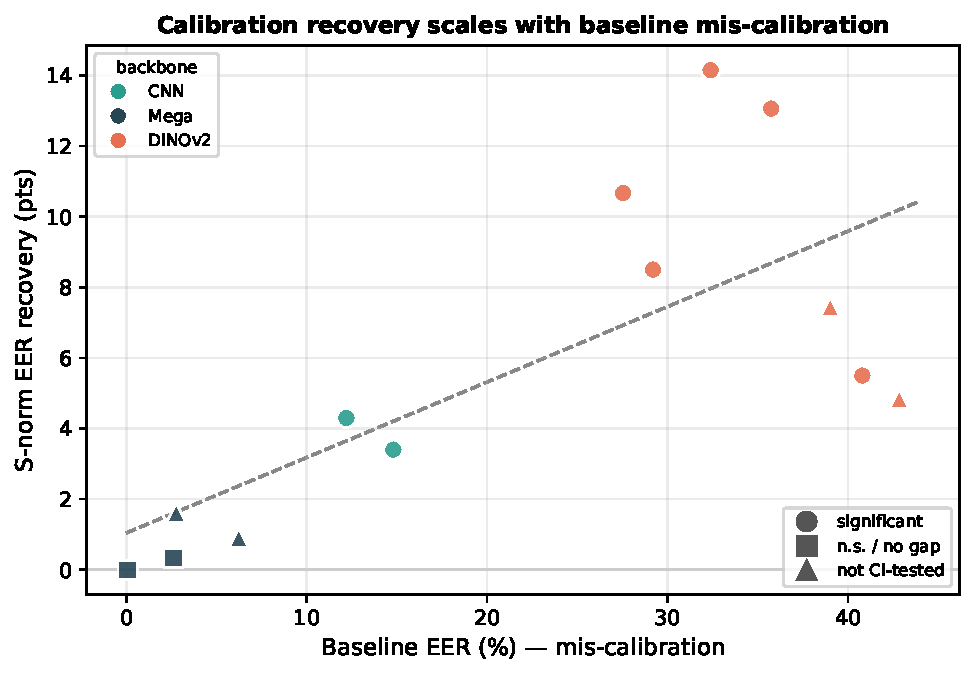
\includegraphics[width=\columnwidth]{fig_calibration_law.pdf}
\caption{The conditional law. S-norm EER recovery grows with the baseline EER (a proxy for score
mis-calibration; trend slope $0.21$). Well-calibrated MegaDescriptor conditions (low EER) cluster at
the bottom-left with negligible, non-significant recovery, while mis-calibrated DINOv2 conditions
(high EER) show large, significant recovery. Marker shape: significant / not-significant or no-gap /
not-CI-tested; colour: backbone.}
\label{fig:law}
\end{figure}

\section{Results}
Table~\ref{tab:main} summarizes recovery across backbones, modalities, and shift families, and
Fig.~\ref{fig:law} visualizes the central finding.

\textbf{The conditional law.} Recovery magnitude and significance track the baseline EER
(Fig.~\ref{fig:law}). Where the
score distribution is well-calibrated (MegaDescriptor on species it was trained on, EER $\approx$
0--3\%), S-norm's effect is small and, on the mild natural panda shift, not significant. Where the
distribution is mis-calibrated (the cattle CNN across datasets, or DINOv2 anywhere), S-norm yields
multi-point, significant EER reductions.

\textbf{Controlled comparison.} On MacaqueFaces with the natural date split, holding data and shift
fixed and varying only the backbone: MegaDescriptor, trained on macaques, is essentially perfect
(0.08\% EER) and gains nothing; DINOv2, never trained for re-ID and mis-calibrated for it, degrades
to 29.2\% EER under the same shift and is significantly recovered by S-norm ($+8.4$ pt, CI
$[+7.2,+9.8]$). Identical inputs, opposite outcomes---the benefit is attributable to backbone
calibration, not the data or the shift.

\textbf{Score-level beats feature-level.} Feature-level AdaBN helped verification on one cattle
cross-dataset but destabilized the other (and collapsed open-set rejection), whereas score-level
S-norm never harmed and helped whenever mis-calibration was present.

\textbf{Negative result on novelty (thoroughly tested).} We asked whether any variant beats plain
S-norm, including in the high-mis-calibration regime (DINOv2) where there is the most headroom. The
outcome is modality-dependent and yields no robust method. A quality-conditioned S-norm significantly
outperforms plain S-norm on face modalities (chimpanzee $+3.3$ pt, macaque $+5.1$--$5.7$ pt, CIs
exclude zero) but is statistically indistinguishable on panda pattern and \emph{significantly worse}
on cattle coat ($-2.7$ pt at high severity). AS-norm and quantile normalization each win on isolated
cases and lose elsewhere. Across datasets no variant reliably beats plain S-norm; we therefore
present the paper as an empirical characterization with plain S-norm as the dependable choice.

\section{Discussion}
Our results reframe a slice of cross-domain re-ID robustness as a calibration question with a
predictable answer. Practitioners deploying a re-ID model to a new site can (i) apply S-norm at
essentially no cost, and (ii) predict whether it will help from the target-set baseline EER before
collecting a single label. That a general model (DINOv2) benefits even in-distribution, while a
specialized model (MegaDescriptor) benefits only under shift, indicates the mechanism is score
mis-calibration rather than domain shift per se---shift is simply one common cause of it.

\textbf{Distributional vs.\ structural calibration.} A consistent pattern explains why plain S-norm
is hard to beat: \emph{distributional} recalibration (S-norm, which normalizes score offsets and
scales) is modality-agnostic and helps whenever mis-calibration is present, whereas \emph{structural}
signals we tested as add-ons---quality conditioning and k-reciprocal re-ranking, which exploit
per-sample confidence or mutual-neighbour topology---help on face modalities but are neutral or
harmful on repetitive patterns (panda coat), where neighbourhood structure is noisy. On MacaqueFaces,
k-reciprocal followed by S-norm reaches 19.3\% EER vs.\ 21.9\% for S-norm alone, yet on IPanda50 the
same combination does not improve over S-norm. A fixed structural prior is thus the wrong
abstraction; a promising direction is a learned test-time module that \emph{gates} structural signals
per input---retaining them where informative (faces) and suppressing them where not (patterns).

\section{Limitations}
(i) The contribution is empirical/analytical; no proposed mechanism robustly outperforms plain
S-norm. (ii) Corruption shifts are controlled proxies; natural shifts are limited to available
metadata. (iii) Jointly learning a calibrator with guarantees is left to future work. (iv) Muzzle
biometrics does not exist for free-ranging wildlife; only the calibration method transfers.

\section{Conclusion}
Cross-domain animal re-identification degradation is, to a first approximation, a score-calibration
problem, and label-free adaptive S-norm is a dependable, zero-cost remedy whose effectiveness is
predictable from a simple mis-calibration signal. We demonstrate this across three backbones, four
modalities, and three shift families, with significance testing and a controlled comparison isolating
calibration as the cause.

\begin{thebibliography}{99}
\bibitem{cermak2024} V.~\v{C}erm\'ak, L.~Picek, L.~Adam, K.~Papafitsoros, ``WildlifeDatasets: An
Open-Source Toolkit for Animal Re-Identification (MegaDescriptor),'' \emph{WACV}, 2024.
\bibitem{oquab2024} M.~Oquab \emph{et al.}, ``DINOv2: Learning Robust Visual Features without
Supervision,'' \emph{TMLR}, 2024.
\bibitem{wang2021} D.~Wang \emph{et al.}, ``Tent: Fully Test-Time Adaptation by Entropy
Minimization,'' \emph{ICLR}, 2021.
\bibitem{li2017} Y.~Li \emph{et al.}, ``Revisiting Batch Normalization for Practical Domain
Adaptation,'' \emph{ICLR Workshop}, 2017.
\bibitem{dart2025} ``DART$^3$: Leveraging Distance for Test-Time Adaptation in Person
Re-Identification,'' 2025.
\bibitem{auckenthaler2000} R.~Auckenthaler, M.~Carey, H.~Lloyd-Thomas, ``Score Normalization for
Text-Independent Speaker Verification Systems,'' \emph{Digital Signal Processing}, 2000.
\bibitem{nandakumar2006} K.~Nandakumar, Y.~Chen, S.~Dass, A.~Jain, ``Quality-based Score Level Fusion
in Multibiometric Systems,'' \emph{ICPR}, 2006.
\bibitem{adam2024} L.~Adam \emph{et al.}, ``WildlifeReID-10k: Wildlife Re-Identification Dataset with
10k Individual Animals,'' 2024.
\bibitem{deng2019} J.~Deng, J.~Guo, N.~Xue, S.~Zafeiriou, ``ArcFace: Additive Angular Margin Loss for
Deep Face Recognition,'' \emph{CVPR}, 2019.
\end{thebibliography}

\end{document}
